% !TeX program = xelatex
\documentclass[10pt,a4paper]{ctexart} % 设置文章类型，正文字号与纸张大小

% 页面与正文常用宏包
\usepackage[margin=2cm]{geometry} % 设置页面四周页边距
\usepackage{graphicx}             % 插入图片
\usepackage{amsmath}              % 提供cases、aligned等数学公式环境
\usepackage{amssymb}              % 提供\therefore等扩展数学符号
\usepackage{booktabs}             % 提供\toprule、\midrule、\bottomrule三线表命令
\usepackage{float}                % 提供[H]固定图片、表格位置
\usepackage{subcaption}           % 提供subfigure子图环境及子图标题
\usepackage{wrapfig}              % 提供wrapfigure图文环绕环境
\usepackage{fancyhdr}             % 自定义页眉和页脚
\usepackage{hyperref}             % 生成超链接

% 页眉页脚
\pagestyle{fancy}                  % 启用fancyhdr定义的页面样式
\fancyhf{}                         % 清空默认页眉和页脚
\fancyfoot[C]{\thepage}            % 在页脚中央显示页码
\renewcommand{\headrulewidth}{0pt} % 隐藏页眉横线
\renewcommand{\footrulewidth}{0pt} % 隐藏页脚横线

% 超链接
\hypersetup{
  colorlinks=true,                % 使用彩色文字链接，而非带边框的链接
  linkcolor=red,                 % 目录、公式及图表交叉引用的颜色
  filecolor=cyan,                 % 本地文件链接的颜色
  urlcolor=blue,                  % 网址链接的颜色
  pdftitle={迈克尔逊干涉仪的应用报告},     % 写入PDF文档属性的标题
  bookmarksnumbered=true          % PDF书签显示章节编号
}

% 定义字号命令
\newcommand{\chuhao}{\fontsize{42pt}{63pt}\selectfont}
\newcommand{\xiaochu}{\fontsize{36pt}{54pt}\selectfont}
\newcommand{\yihao}{\fontsize{26pt}{39pt}\selectfont}
\newcommand{\xiaoyi}{\fontsize{24pt}{36pt}\selectfont}
\newcommand{\erhao}{\fontsize{22pt}{33pt}\selectfont}
\newcommand{\xiaoer}{\fontsize{18pt}{27pt}\selectfont}
\newcommand{\sanhao}{\fontsize{16pt}{24pt}\selectfont}
\newcommand{\xiaosan}{\fontsize{15pt}{22.5pt}\selectfont}
\newcommand{\sihao}{\fontsize{14pt}{21pt}\selectfont}
\newcommand{\xiaosi}{\fontsize{12pt}{18pt}\selectfont}
\newcommand{\wuhao}{\fontsize{10.5pt}{15.75pt}\selectfont}
\newcommand{\xiaowu}{\fontsize{9pt}{13.5pt}\selectfont}

% 章节格式
\ctexset{
  section={
    format={\CJKfontspec[AutoFakeBold=2.5]{KaiTi}\sanhao\bfseries}, % 一级标题使用三号加粗楷体
    name={,、},                                                    % 在中文章节序号后添加顿号
    number=\chinese{section},                                      % 一级标题编号使用“一、二、三”形式
    aftername={}                                                   % 取消编号与标题文字之间的空格
  },
  subsection={
    format={\CJKfontspec[AutoFakeBold=2.5]{KaiTi}\sihao\bfseries}, % 二级标题使用四号加粗楷体                                               
  },
  subsubsection={
    format={\CJKfontspec[AutoFakeBold=2.5]{KaiTi}\xiaosi\bfseries}, % 三级标题使用小四加粗楷体
  }
}

\begin{document}

% 封面
\thispagestyle{fancy} % 封面保留底部居中的页码
\fancyfoot[C]{\thepage}
\begin{center}
  \CJKfontspec[AutoFakeBold=2.5]{KaiTi}\bfseries % 封面中文使用楷体并人工加粗，西文同时加粗
  \vspace{0.8cm}
  
\includegraphics[width=8.2cm]{figures/head.png}

  \vspace{0.2cm}
  \xiaochu 
    物理实验报告

  \vspace{3.5cm}
  \begin{minipage}{10.0cm}
    \sanhao
    \makebox[2.6cm][l]{实验名称：}
    \underline{\makebox[7.0cm][c]{迈克尔逊干涉仪的应用}}\par\vspace{12pt}

    \makebox[2.6cm][l]{实验桌号：}
    \underline{\makebox[7.0cm][c]{8}}\par\vspace{12pt}

    \makebox[2.6cm][l]{指导教师：}
    \underline{\makebox[7.0cm][c]{包泽杭}}
  \end{minipage}

  \vspace{3.5cm}
  \begin{minipage}{10.0cm}
    \sihao
    \makebox[1.4cm][l]{班级：}
    \underline{\makebox[8.0cm][c]{}}\par\vspace{10pt}

    \makebox[1.4cm][l]{姓名：}
    \underline{\makebox[8.0cm][c]{IllusoryRain}}\par\vspace{10pt}

    \makebox[1.4cm][l]{学号：}
    \underline{\makebox[8.0cm][c]{}}
  \end{minipage}

  \vspace{2.0cm}
  \sihao
    实验日期：
    \underline{\makebox[0.7cm][c]{2026}}年
    \underline{\makebox[0.7cm][c]{11}}月
    \underline{\makebox[0.7cm][c]{25}}日
    星期\underline{\makebox[0.7cm][c]{三}}上午

  \vspace{0.7cm}
  \sihao 
    浙江大学物理实验教学中心
\end{center}

\newpage
\xiaosi\songti\mdseries % 后续正文统一使用小四不加粗的宋体

\section{预习报告（10分）}

  \subsection{实验综述（5分）}

    \subsubsection{光的干涉条件}
    两束光频率相同、振动方向一致、相位差恒定，且光程差在相干长度内时，可形成稳定干涉条纹。光程差满足
    \[
    \delta=k\lambda\quad\text{时干涉加强},\qquad
    \delta=\left(k+\frac{1}{2}\right)\lambda\quad\text{时干涉相消},
    \qquad k\in\mathbb{Z}
    \]

    \subsubsection{获取相干光的两种途径}
    将同一光源的光分成两束后重新叠加：分波面法分割同一波阵面；分振幅法利用反射与透射分光，迈克尔逊干涉仪采用后者。

    \begin{figure}[H]
      \centering
      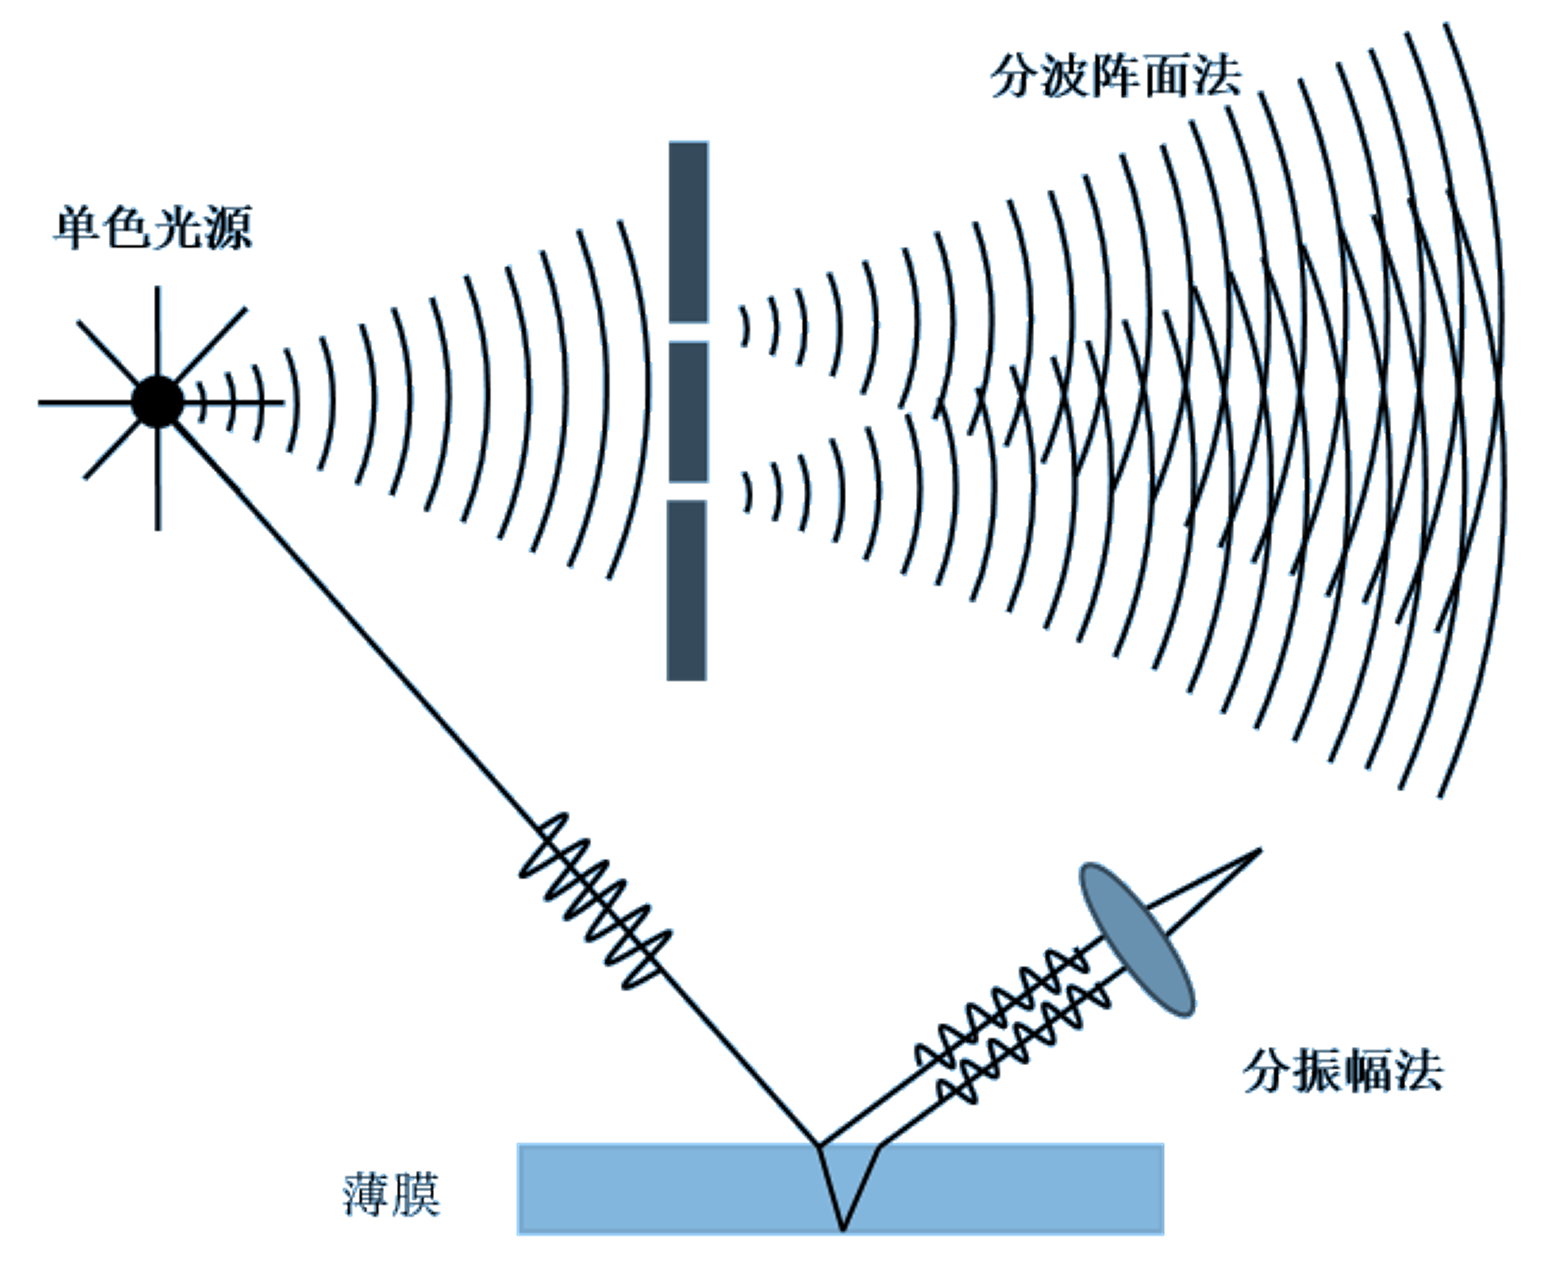
\includegraphics[width=0.4\textwidth]{figures/图1.png}
      \caption{获取相干光的两种途径}
    \end{figure}

    \subsubsection{迈克尔逊干涉仪光路}
    分光镜P1将入射光分成两束，经两反射镜返回后汇合干涉；补偿板P2使两束光在玻璃中通过的光程相同。调节反射镜的倾角和位置，可改变条纹形状与光程差。

    \begin{figure}[H]
      \centering
      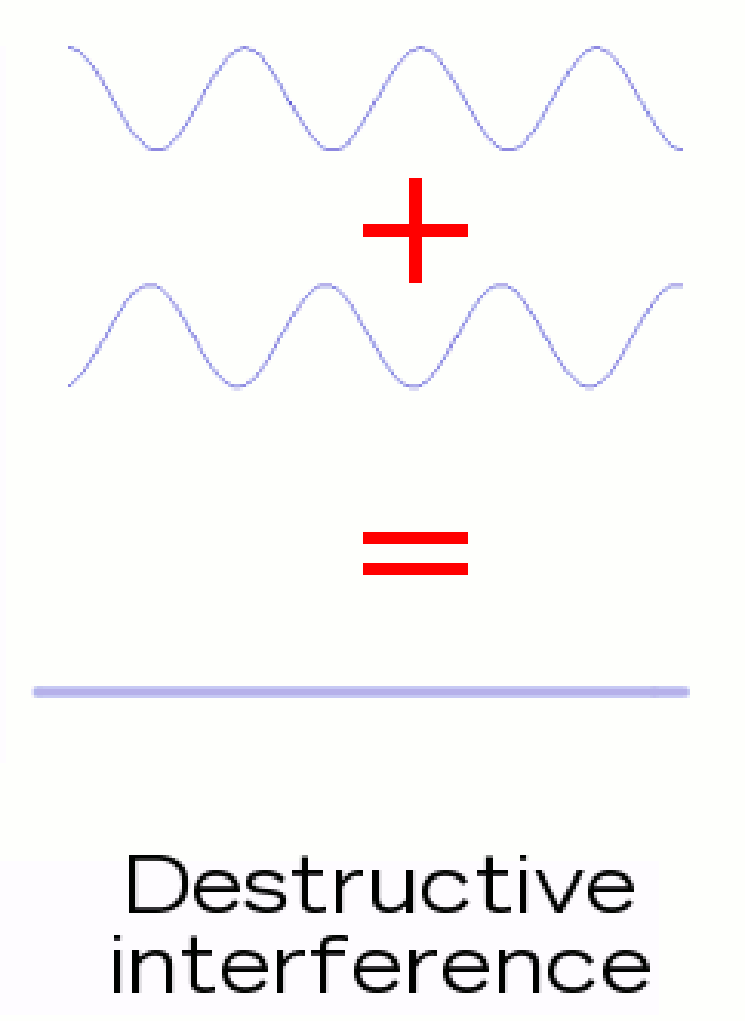
\includegraphics[width=0.4\textwidth]{figures/图2.png}
      \caption{迈克尔逊干涉仪光路图}
    \end{figure}

    \subsubsection{定域等倾干涉}
    两等效反射面平行、间距为$d$时，倾角为$\theta$的光线光程差为
    \[
    \delta=2d\cos\theta,\qquad
    2d\cos\theta_k=k\lambda\quad\text{（亮纹）}
    \]
    
    相同倾角对应同一条纹，形成定域于无穷远的同心圆环。

    \subsubsection{钠光波长的测定}
    单向移动动镜$\Delta d$，中心吞吐$N$个圆环时，光程差改变$2\Delta d=N\lambda$，故
    \[
    \boxed{\lambda=\frac{2\Delta d}{N}}
    \]

    \subsubsection{钠黄双线波长差的测定}
    钠黄双线波长约为$589.0\,\mathrm{nm}$和$589.6\,\mathrm{nm}$，两组条纹叠加使可见度周期性变化。相邻两次可见度最小时，动镜位移$\Delta d$满足
    \[
    \boxed{\Delta\lambda\approx\frac{\bar{\lambda}^{\,2}}{2\Delta d}},
    \qquad \bar{\lambda}=\frac{\lambda_1+\lambda_2}{2}
    \]

    \begin{figure}[H]
      \centering
      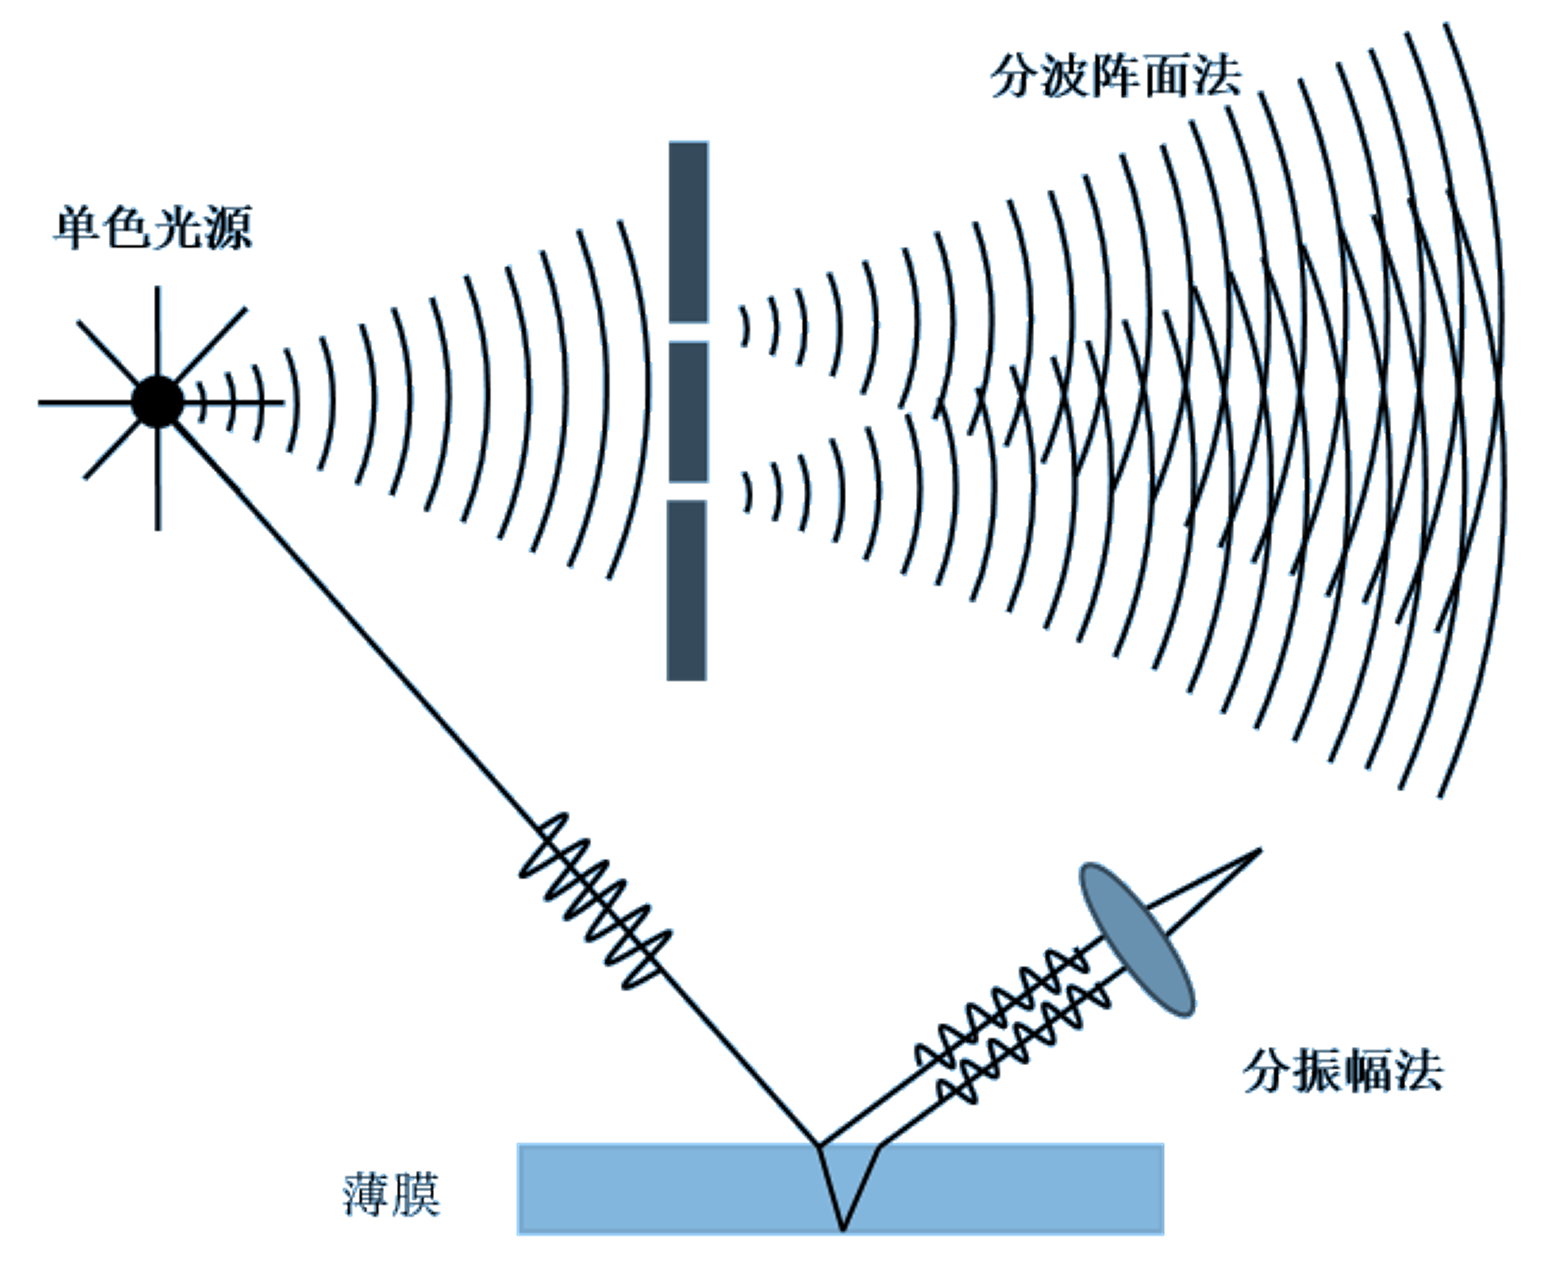
\includegraphics[width=0.4\textwidth]{figures/图3.png}
      \caption{钠黄双线波长差的测定}
    \end{figure}

    \begin{samepage}
    \subsubsection{实验内容}
    调出清晰、稳定的等倾圆环条纹，用CCD观察，并保持动镜单向移动。
    \begin{enumerate}
      \item 测量钠光波长：每吞吐50个圆环记录一次动镜位置，由位移与环数计算波长。
      \item 测量双线波长差：连续记录至少3次条纹可见度最小时的动镜位置，由相邻位置之差计算双线波长差。
    \end{enumerate}
    \end{samepage}

  \subsection{实验重点（3分）}
  \begin{enumerate}
    \item 了解迈克尔逊干涉仪的结构并掌握调节方法；
    \item 观察光波干涉现象，加深对干涉理论的理解；
    \item 理解定域干涉与非定域干涉；
    \item 测量钠光波波长。
  \end{enumerate}

  \subsection{实验难点（2分）}
  \begin{enumerate}
    \item 调节光路，使两束光重合并获得清晰、稳定的圆环条纹；
    \item 准确计数中心环纹的涌出或陷入，并读取动镜位移以测定钠光波长；
    \item 判断条纹可见度最小的位置，测定钠黄双线的波长差。
  \end{enumerate}

\section{实验操作与原始数据（50分）}
% 填写自己的实验数据图，这个实验我做的依托，这个报告当做一个反面教材阅读比较好

\section{结果与分析（30分）}

  \subsection{数据处理与结果（20分）}
  本次实验中，由于首台迈克尔逊干涉仪经老师检查，存在螺丝松动问题，
  且测量后期干涉条纹较为模糊，所以我根据老师指导选择记录了两组数据。
  第一组包含9个动镜位置读数，依旧采用跨6个记录间隔的逐差法；
  第二组则采用平均法处理，由于最后一个读数$d_4$因测量时条纹过于模糊，读数不可靠，误差过大而略去，
  仅保留在原始记录中，不参与后续数据分析。

  \subsubsection{位移与波长的换算}
  实验中，每吞吐或者形成50条干涉条纹记录一次动镜位置。
  由$N\lambda=2\Delta d$，
  得到每个记录间隔对应的波长为$\lambda=\Delta d/25$，故
  \[
    \frac{\lambda_i}{\mathrm{nm}}
    =\frac{10^6}{25}\frac{\Delta d_i}{\mathrm{mm}}
  \]

  数据最终结果呈现时，位置读数、位移差及平均位移均保留五位小数，波长保留一位小数，
  但中间计算会使用未修约数值，以此提高处理精度。

  \subsubsection{第一组：逐差法}
  对$d_7-d_1$、$d_8-d_2$和$d_9-d_3$分别除以6，得到每50条条纹对应的动镜位移：
  \[
    \Delta d_i=\frac{d_{i+6}-d_i}{6},\qquad i=1,2,3
  \]
  
  其中$d_4$、$d_5$、$d_6$仅保留在表中，不参与逐差计算，而之后的线性回归将会使用全部9个读数。

  \begin{table}[H]
    \centering
    \caption{钠光波长测定第一组数据}
    \label{tab:wavelength-first}
    \begin{tabular}{ccccc}
      \toprule
      \multicolumn{2}{c}{动镜位置 $d_i/\mathrm{mm}$}
      & $\Delta d_i/\mathrm{mm}$ & $\lambda_i/\mathrm{nm}$ & $\bar{\lambda}/\mathrm{nm}$ \\
      \midrule
        $d_1=50.53400$ & $d_7=50.63673$ & 0.01712 & 684.9 & 674.7 \\
        $d_2=50.55148$ & $d_8=50.65225$ & 0.01680 & 671.8 &  \\
        $d_3=50.56799$ & $d_9=50.66810$ & 0.01669 & 667.4 &  \\
        $d_4=50.58432$ & & & & \\
        $d_5=50.60055$ & & & & \\
        $d_6=50.62040$ & & & & \\
      \bottomrule
    \end{tabular}
  \end{table}

  上表中最后一列为计算所得整组平均值。即由3组逐差位移得到
  \[
    \overline{\Delta d}^{(1)}=0.01687\,\mathrm{mm},\qquad
    \bar\lambda^{(1)}=674.7\,\mathrm{nm}
  \]

  \subsubsection{第二组：平均值法}
  第二组实验因为是逆时针转动动镜，因此位置随条纹计数增加而减小，数据处理时取有效相邻读数差的绝对值：
  \[
    \Delta d_i=|d_i-d_{i-1}|,\qquad i=2,3
  \]

  \begin{table}[H]
    \centering
    \caption{钠光波长测定第二组数据}
    \label{tab:wavelength-second}
    \begin{tabular}{cccc}
      \toprule
      动镜位置 $d_i/\mathrm{mm}$ & $\Delta d_i/\mathrm{mm}$
      & $\lambda_i/\mathrm{nm}$ & $\bar{\lambda}/\mathrm{nm}$ \\
      \midrule
        $d_1=50.48100$ & & & 585.8 \\
        $d_2=50.46635$ & 0.01465 & 586.0 & \\
        $d_3=50.45171$ & 0.01464 & 585.6 & \\
        $d_4=50.43349$ & & & \\
      \bottomrule
    \end{tabular}
  \end{table}

  最后一行$d_4$仅作记录，因条纹过于模糊而不参与计算。其余两段位移的平均值为
  \[
    \overline{\Delta d}^{(2)}
    =\frac{0.01465+0.01464}{2}
    \approx 0.01465\,\mathrm{mm},\qquad
    \bar\lambda^{(2)}=585.8\,\mathrm{nm}
  \]
  
  \begin{figure}[H]
    \centering
    \begin{minipage}{0.4\textwidth}
      \centering
      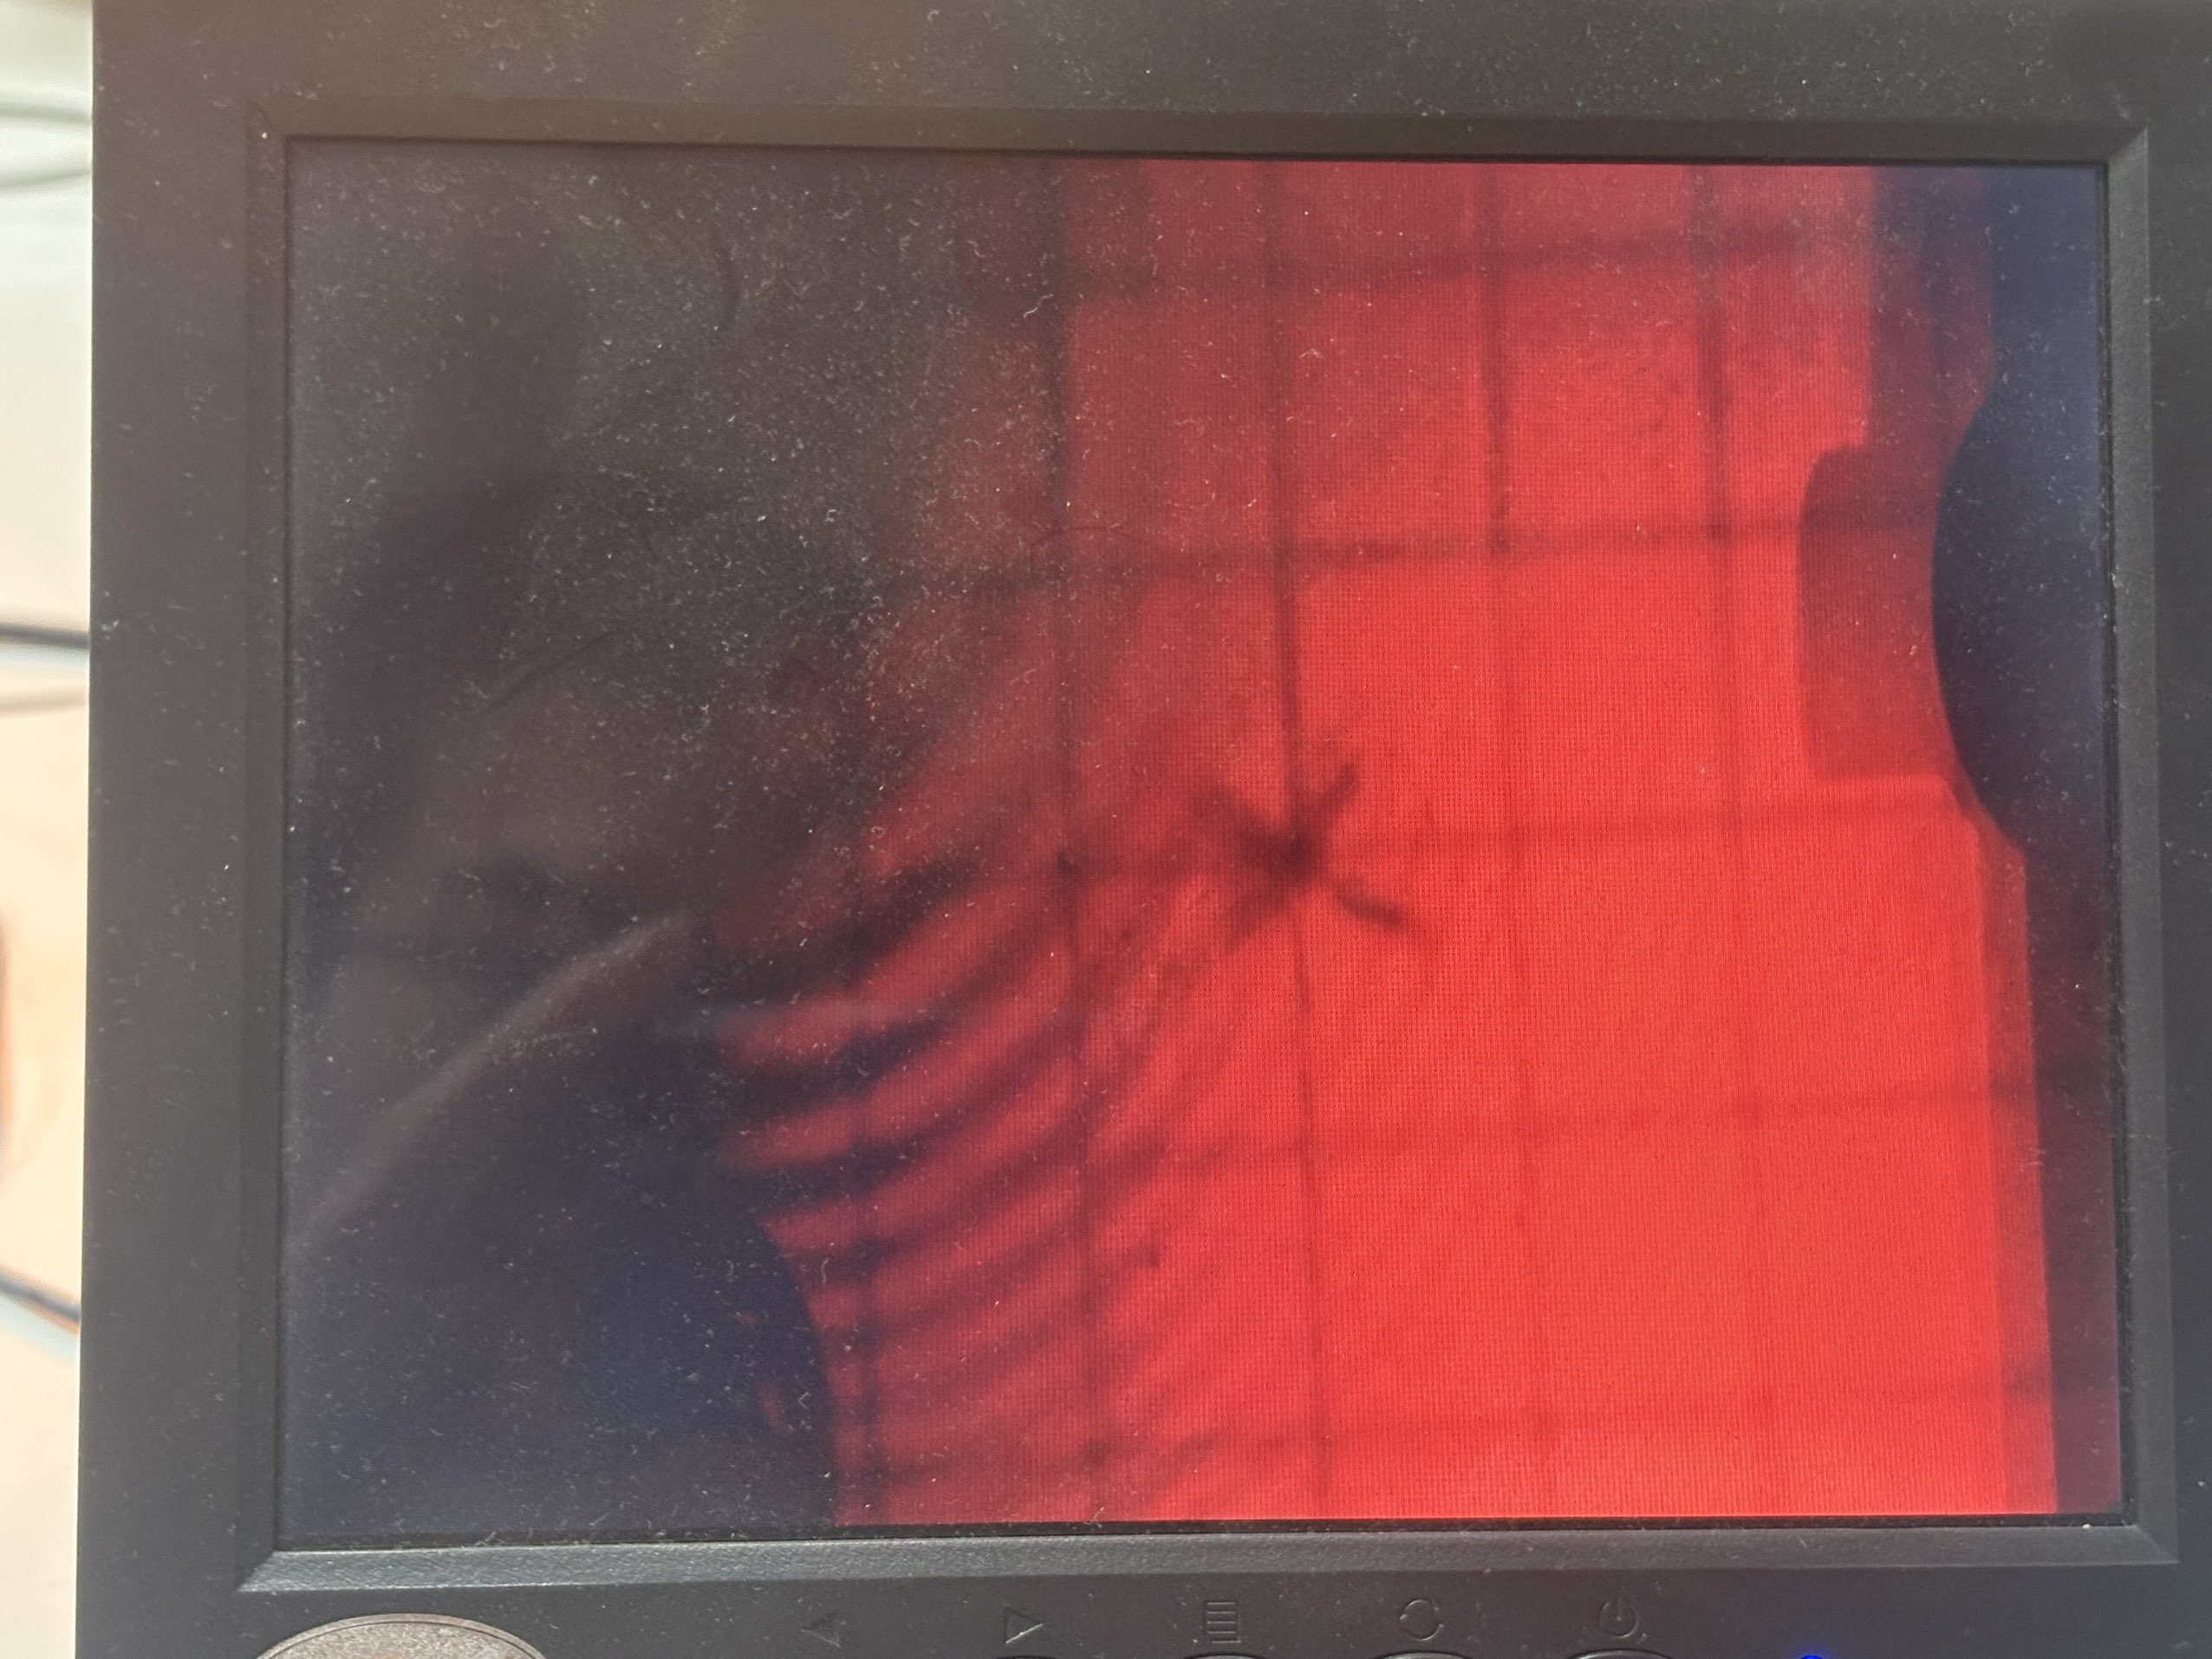
\includegraphics[width=\linewidth]{figures/图5.png}
      \caption{第一组数据的干涉条纹}
    \end{minipage}
    \hfill
    \begin{minipage}{0.4\textwidth}
      \centering
      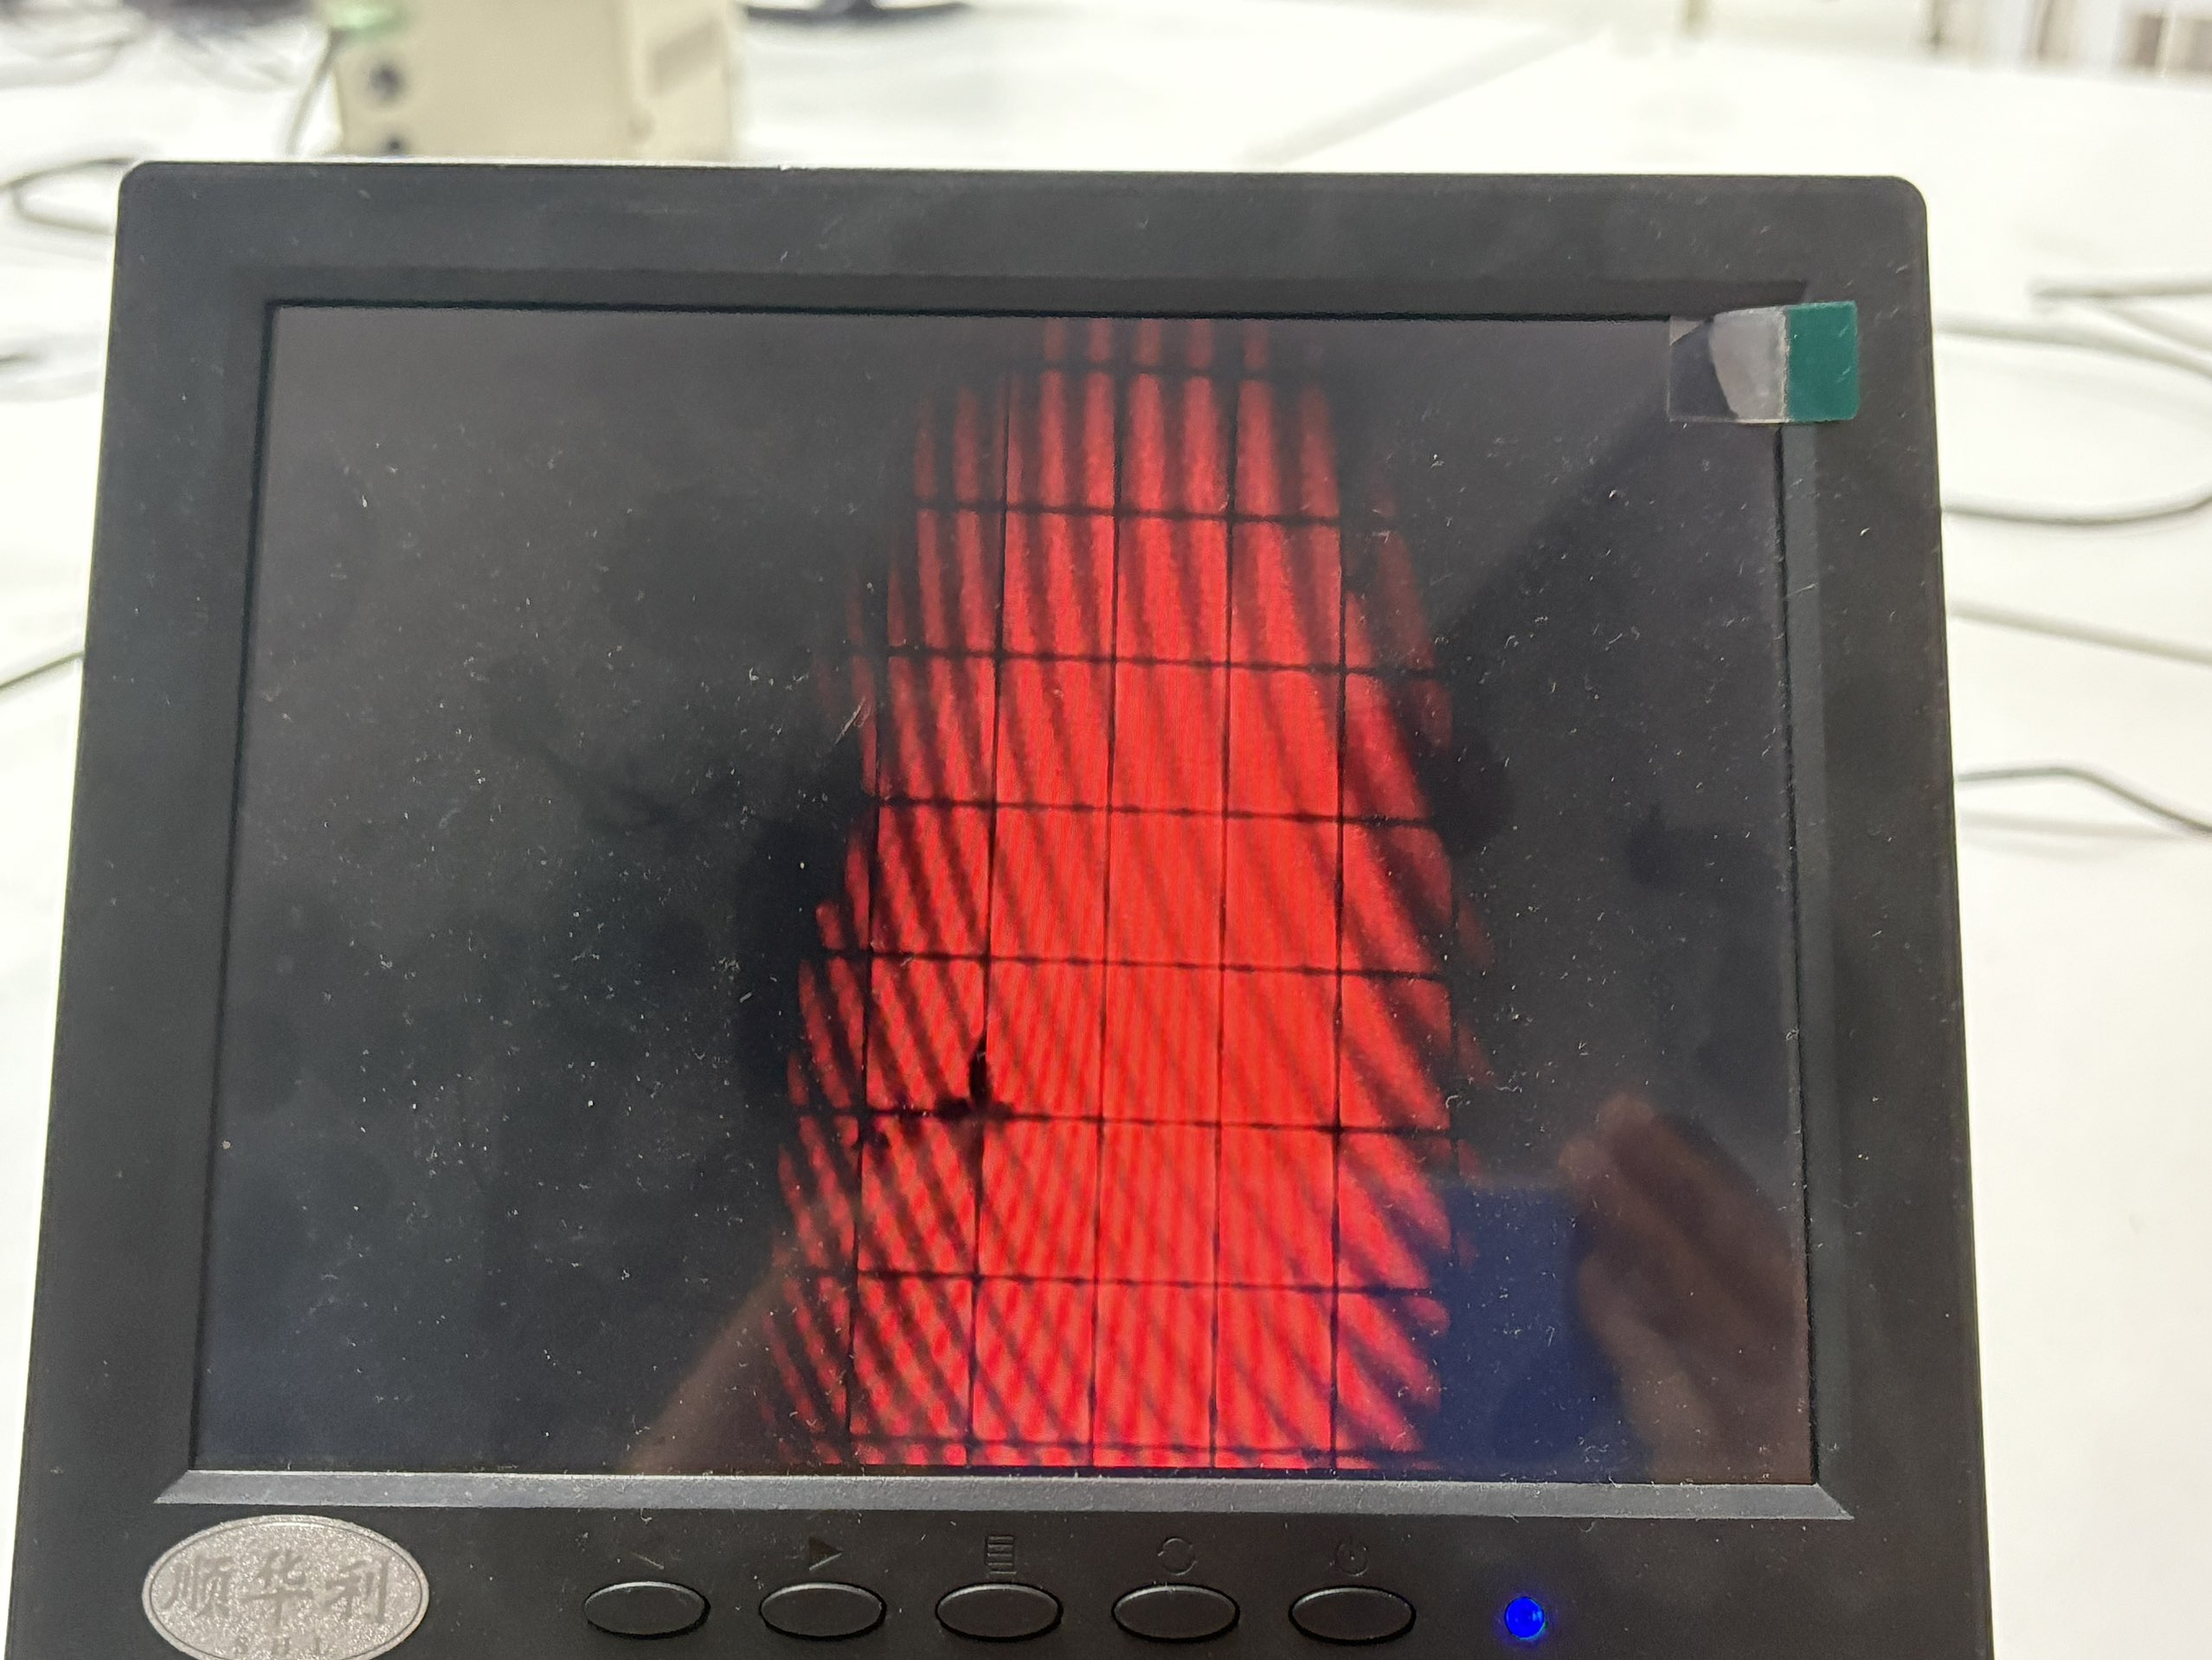
\includegraphics[width=\linewidth]{figures/图6.png}
      \caption{第二组数据的干涉条纹}
    \end{minipage}
  \end{figure}

  \subsubsection{线性回归法}
  对两组都进行线性回归分析，每组都以首个读数为计数起点，令$N_i=50(i-1)$，分别作一元线性回归：
  \[
    d=kN+b,\qquad
    \frac{\lambda_{\mathrm{fit}}}{\mathrm{nm}}
    =2\left|\frac{k}{\mathrm{mm}/\text{条}}\right|\times10^6
  \]

  其中第一组使用全部9个读数，第二组则使用$d_1,d_2,d_3$，略去$d_4$。拟合结果表格和图如下：
  
  \begin{table}[H]
    \centering
    \caption{线性回归结果}
    \begin{tabular}{ccccc}
      \toprule
      数据组 & $k/(\mathrm{mm}/\text{条})$ & $b/\mathrm{mm}$ & $R^2$
      & $\lambda_{\mathrm{fit}}/\mathrm{nm}$ \\
      \midrule
      第一组 & $3.3742333\times10^{-4}$ & 50.53427 & 0.99953548 & 674.8 \\
      第二组 & $-2.9290000\times10^{-4}$ & 50.48100 & 0.99999996 & 585.8 \\
      \bottomrule
    \end{tabular}
  \end{table}

  \begin{figure}[H]
    \centering
    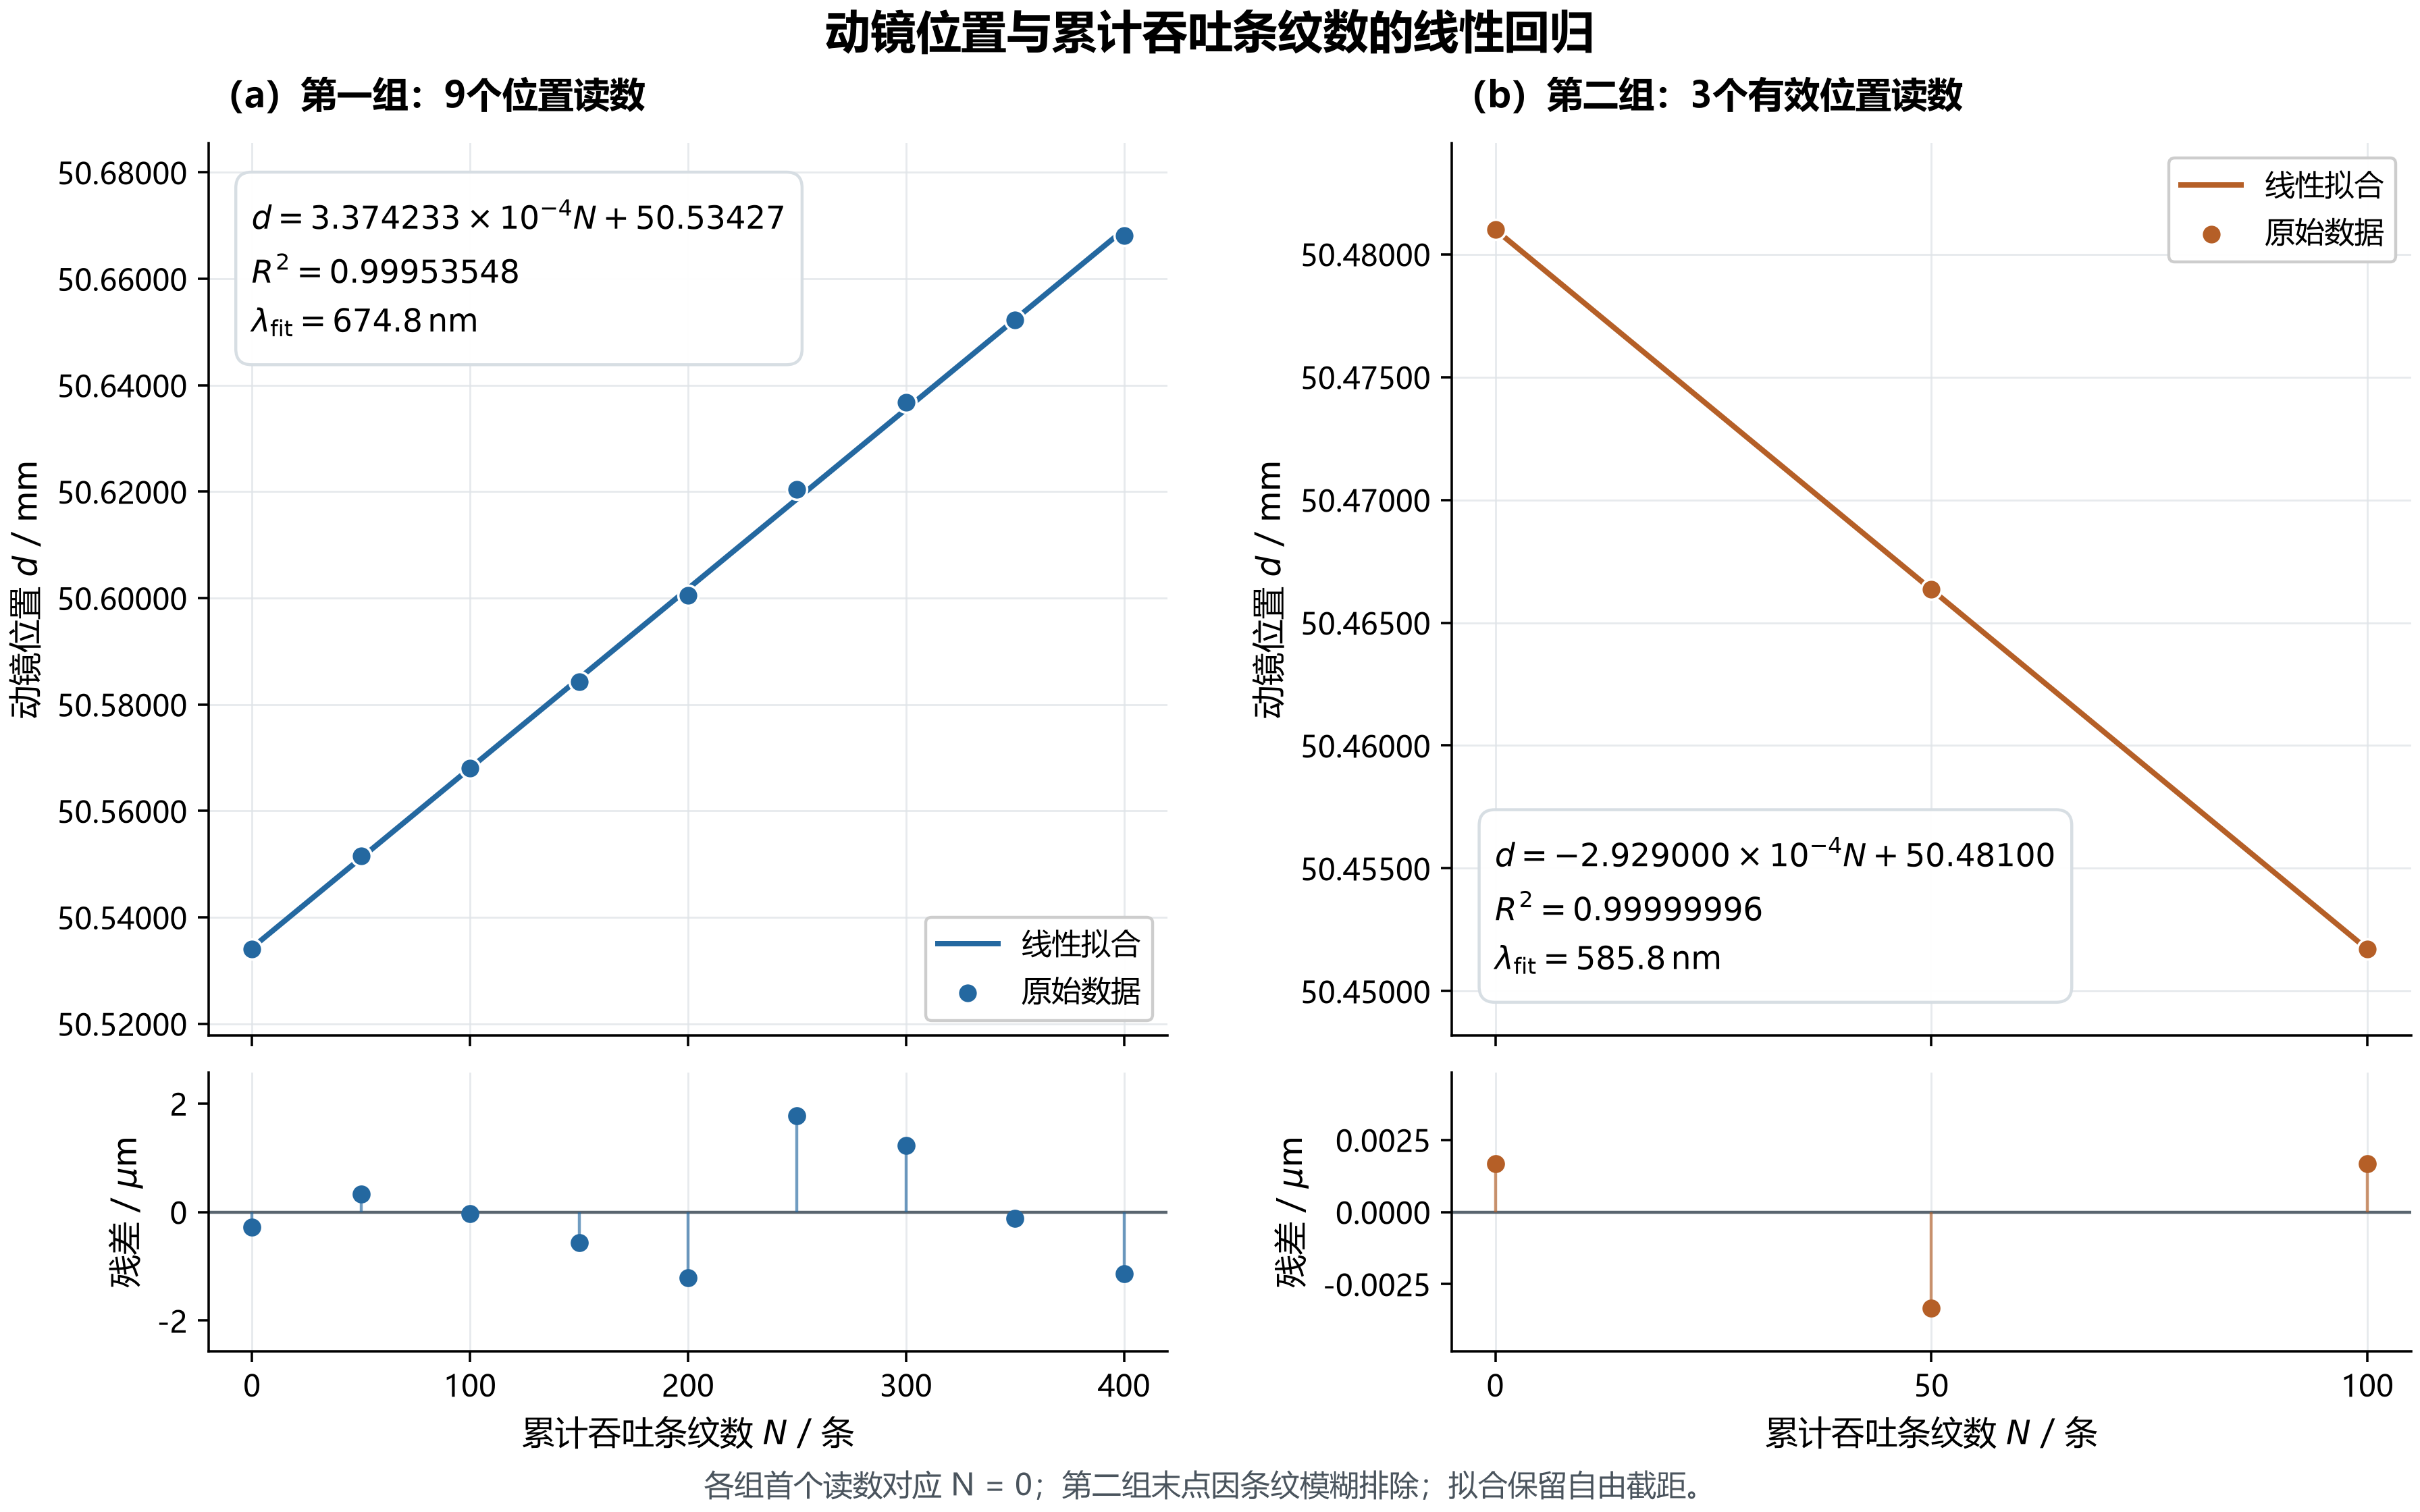
\includegraphics[width=0.8\textwidth]{figures/图7.png}
    \caption{两组有效动镜位置与累计吞吐条纹数的线性拟合及残差}
  \end{figure}

  由图7可见，两组动镜位置与累计条纹数均近似呈线性关系，斜率正负对应动镜移动方向。
  第一组虽有较高的$R^2$，但残差波动明显，拟合波长$674.8\,\mathrm{nm}$仍显著偏高，说明线性相关性好但并不代表测量准确。
  第二组有效点的残差较小，拟合波长$585.8\,\mathrm{nm}$与平均值法一致，但仅有3个有效点，实际上需要增加测量次数以检验稳定性。

  \subsubsection{不确定度与最终结果}
  平均位移的A类标准不确定度计算公式为
  \[
    u_A(\overline{\Delta d})
    =\sqrt{\frac{\sum_{i=1}^{m}(\Delta d_i-\overline{\Delta d})^2}{m(m-1)}}
  \]

  第一组采用3组逐差位移，代入未修约数据得
  \[
    u_A^{(1)}(\overline{\Delta d})
    =\sqrt{\frac{\sum_{i=1}^{3}(\Delta d_i-\overline{\Delta d}^{(1)})^2}{3\times2}}
    =1.3\times10^{-4}\,\mathrm{mm}
  \]

  第二组采用2段有效相邻位移，代入未修约数据得
  \[
    u_A^{(2)}(\overline{\Delta d})
    =\sqrt{\frac{\sum_{i=2}^{3}(\Delta d_i-\overline{\Delta d}^{(2)})^2}{2\times1}}
    =5.0\times10^{-6}\,\mathrm{mm}
  \]

  按照本次实验要求，将$\Delta d$作为直接测量量，取仪器误差限$a=0.00005\,\mathrm{mm}$，
  按均匀分布计算两组相同的B类标准不确定度：
  \[
    u_B^{(1)}(\overline{\Delta d})=u_B^{(2)}(\overline{\Delta d})
    =\frac{a}{\sqrt3}=2.9\times10^{-5}\,\mathrm{mm}
  \]
  
  将A、B类分量合成，得到平均位移的合成标准不确定度：
  \[
    u_c(\overline{\Delta d})
    =\sqrt{u_A^2(\overline{\Delta d})+u_B^2(\overline{\Delta d})}
  \]

  忽略条纹计数的不确定度，由$\lambda=\Delta d/25$换算波长的不确定度：
  \[
    \frac{u_c(\lambda)}{\mathrm{nm}}
    =\frac{10^6}{25}\frac{u_c(\overline{\Delta d})}{\mathrm{mm}}
  \]

  最终得到两组的不确定度计算结果汇总如下：
  \begin{table}[H]
    \centering
    \caption{两组测量结果的标准不确定度}
    \begin{tabular}{ccc}
      \toprule
      计算量 & 第一组 & 第二组 \\
      \midrule
      $u_A(\overline{\Delta d})/\mathrm{mm}$ & $1.3\times10^{-4}$ & $5.0\times10^{-6}$ \\
      $u_B(\overline{\Delta d})/\mathrm{mm}$ & $2.9\times10^{-5}$ & $2.9\times10^{-5}$ \\
      $u_c(\overline{\Delta d})/\mathrm{mm}$ & $1.3\times10^{-4}$ & $2.9\times10^{-5}$ \\
      $u_A(\lambda)/\mathrm{nm}$ & 5.2 & 0.2 \\
      $u_B(\lambda)/\mathrm{nm}$ & 1.2 & 1.2 \\
      $u_c(\lambda)/\mathrm{nm}$ & 5.4 & 1.2 \\
      \bottomrule
    \end{tabular}
  \end{table}

  对波长及其标准不确定度保留一位小数，最终结果为
  \[
    \boxed{\lambda^{(1)}=(674.7\pm5.4)\,\mathrm{nm}},\qquad
    \boxed{\lambda^{(2)}=(585.8\pm1.2)\,\mathrm{nm}}
  \]

  以$589.3\,\mathrm{nm}$为参考值，第一、二组平均波长的相对偏差分别为$14.49\%$和$0.59\%$。
  对于第一组的误差为什么会如此大，后续的误差分析中将进行讨论。

  \subsection{误差分析（10分）}
  根据上述数据分析，可以发现：
  第一组平均波长偏高，相对偏差为$14.49\%$，各段位移波动较大；第二组有效数据重复性较好，相对偏差降至$0.59\%$。
  
  主要误差来源如下：
  \begin{enumerate}
    \item 仪器螺丝松动：第一组测量后，老师检查发现仪器螺丝松动，可能使镜架或传动结构不稳，造成示值与实际位移不一致，是第一组较大偏差的重要可能来源。
    \item 条纹计数与终点判断：每段需连续计数50个条纹，条纹模糊或视觉疲劳易引起漏计、错计及终点判断偏差。
    比如第二组最后一点$d_4$就是典型的因条纹模糊、读数不可靠而产生的不可靠数据。
    \item 空程、估读与振动：反向转动手轮可能引入空程，鼓轮估读和实验台微振也会增加读数分散性，测量时应保持单向转动并减小扰动。
  \end{enumerate}

\section{实验探讨与思考题（10分）}

  \subsection{实验探讨}
  本次实验让我体会到，精密光学测量尤其需要耐心。
  调节摄像头和反射镜时，需反复微调、观察，才能获得清晰稳定的条纹；
  连续计数50个条纹时，要保持专注，避免因急躁而漏计或误判。
  面对较大误差，应保留原始数据，复核计算，结合仪器状态与操作过程分析原因，必要时复测，而不能随意删改数据。
  反思本次实验，我对仪器检查和条纹模糊时的处理仍不够细致。
  今后应提前检查仪器，调节时循序渐进，测量中及时核验结果。

  \subsection{思考题}

    \subsubsection{如何判断\texorpdfstring{$M_1'$}{M1'}与\texorpdfstring{$M_2$}{M2}是否平行？}
    用扩展钠光源照明，微调反射镜倾角，直至出现清晰、完整的同心圆环。
    缓慢移动动镜，若圆环围绕同一圆心收缩或扩张，说明两等效反射面基本平行；若呈直条纹或明显偏离圆形，则需继续调节。

    \subsubsection{如何找零光程位置？}
    先用钠光调出等倾圆环，沿圆环向中心收缩的方向移动动镜，使条纹变粗、变疏。
    再使两等效镜面略有夹角，换用白光微调，寻找零光程差附近的彩色条纹，由中央消色条纹确定等光程位置。

    \subsubsection{什么原因形成空程？在测量中如何避免引入空程？}
    空程源于丝杆、螺母等传动部件的机械间隙，反向转动时需先消除间隙，动镜才开始移动。
    测量前沿选定方向转动，待条纹稳定吞吐后记录起点，此后保持单向转动。
    若越过目标，应退回足够距离，再沿原方向接近读数。

\vspace*{\fill} % 使下面内容在页面底部显示
\noindent
\begin{minipage}{\textwidth}
  注意事项：

  \begingroup
    \setlength{\leftskip}{2em} % 1--4整体向右缩进两个汉字宽度
    1. 用PDF格式上传“实验报告”，文件名：学生姓名+学号+实验名称+周次。

    2. “实验报告”必须递交在“学在浙大”本课程内对应实验项目的“作业”模块内。

    3. “实验报告”成绩必须在“浙江大学物理实验教学中心网站”-“选课系统”内查询。

    4. 教学评价必须在“浙江大学物理实验教学中心网站”-“选课系统”内进行，学生必须进行教学评价，才能看到实验报告成绩，教学评价须在本次实验结束之后3天内进行。\par
  \endgroup

  \begin{center}
    {\CJKfontspec[AutoFakeBold=2.5]{SimSun}\bfseries 浙江大学物理实验教学中心制}
  \end{center}
\end{minipage}

\end{document}
